\documentclass{report}
\usepackage[utf8]{inputenc}
\usepackage{fixlatvian}
\usepackage{tabularx}
\usepackage{graphicx}
\usepackage{verbatim}
\usepackage{caption}
\usepackage[siunitx, europeanresistors, americaninductors, oldvoltagedirection]{circuitikz}
\usepackage{pgfplots}
\pgfplotsset{compat=1.15}

\title{Vienkāršu elektrisku shēmu modelēšana}
\author{Dāvis Daniels Anstrangs 171REB155}
\date{09.03.2018}

\begin{document}

\maketitle

\chapter{Teorētiskā daļa}
\section{Ķēdes aprēķins}
Jāaprēķina spriegums uz rezistoriem, kuri doti shēmā. Par sprieguma avota vērtību tiek ņemti pēdējie trīs apliecības cipar dalīti ar 10. Bet rezistoru vērtības ir ņemtas tā, ka R1 ir pirmspēdējā cipara vērtība+1, bet R2 ir pēdējā cipara vērtība+1. 
\begin{equation}
I=\frac{U}{R}
\end{equation}\label{eq:1}
Oma likums(\ref{eq:1}) kā dots literatūrā\cite{Oms}.
\begin{equation}
I=\frac{U}{R1+R2}
\end{equation}
\begin{equation}
U_{R1}=I*R_1
\end{equation}
\begin{equation}
U_{R2}=I*R_2
\end{equation}

\begin{figure}[b]
\centering
\begin{tabular}{|c|r|}
\hline
R1 & 6 $\Omega$\\
\hline
R2 & 6 $\Omega$\\
\hline
V1 & 15.5V\\
\hline
$U_{R1}$ & 7.75V\\
\hline
$U_{R2}$ & 7.75V\\
\hline
\end{tabular}
\captionof{table}{Tabula ar uzdotajiem datiem}\label{tab:1}
\end{figure}

\begin{figure}
\centering
\begin{circuitikz}[scale=1, every node/.style={transform shape}]
\draw
(0,2) to[R=$R1$, -] (4,2)
(4,2) to[R=$R2$, -] (4,0)
(0,0) to[short, -] (4,0)
(0,0) to[american voltage source, v<=$V1$, -] (0,2) 
;
\end{circuitikz}
\caption{Dotās shēmas attēlojums ar "circuitikz" pakas palīdzību.}\label{sch:1}
\end{figure}

\begin{figure}
\begin{center}
\begin{tikzpicture}
\begin{axis}[
    xlabel=$R2$,
    ylabel=$U_{R2}$
    ]
\addplot[color=blue,mark=o] coordinates {
		(5,7.05)
		(10,9.69)
		(15,11.1)
		(20,11.9)
		(25,12.5)
		(30,12.9)
		(35,13.2)
		(40,13.5)
		(45,13.7)
		(50,13.8)
	};
\end{axis}
\end{tikzpicture}
\caption{$U_{R2}$=\textit{f}(\textit{R2}) grafiks, pēc sweep simulācijas datiem.}\label{graph:1}
\end{center}
\end{figure}


\chapter{Praktiskā daļa}
\section{Darbs ar GEDA programmām}
\subsection{Darbs ar gschem}
Shēma redzama \ref{att:1} attēlā

\begin{figure}[b!]
\centering
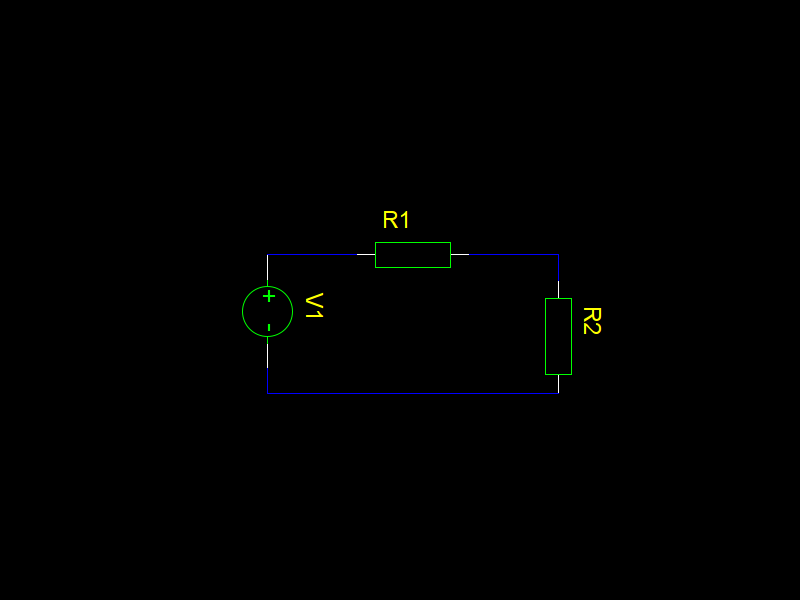
\includegraphics[width=9cm]{01.png}
\captionof{figure}{gschem shēma}
\label{att:1}
\end{figure}

\newpage
\subsection{Darbs ar gnetlist}
\begin{verbatim}
* Spice netlister for gnetlist
R2 2 0 6
R1 1 2 6
V1 1 0 15.5
.END
\end{verbatim}
\subsection{Darbs ar ngspice}

\begin{figure}[b!]
\centering
\begin{minipage}{.5\textwidth}
\centering
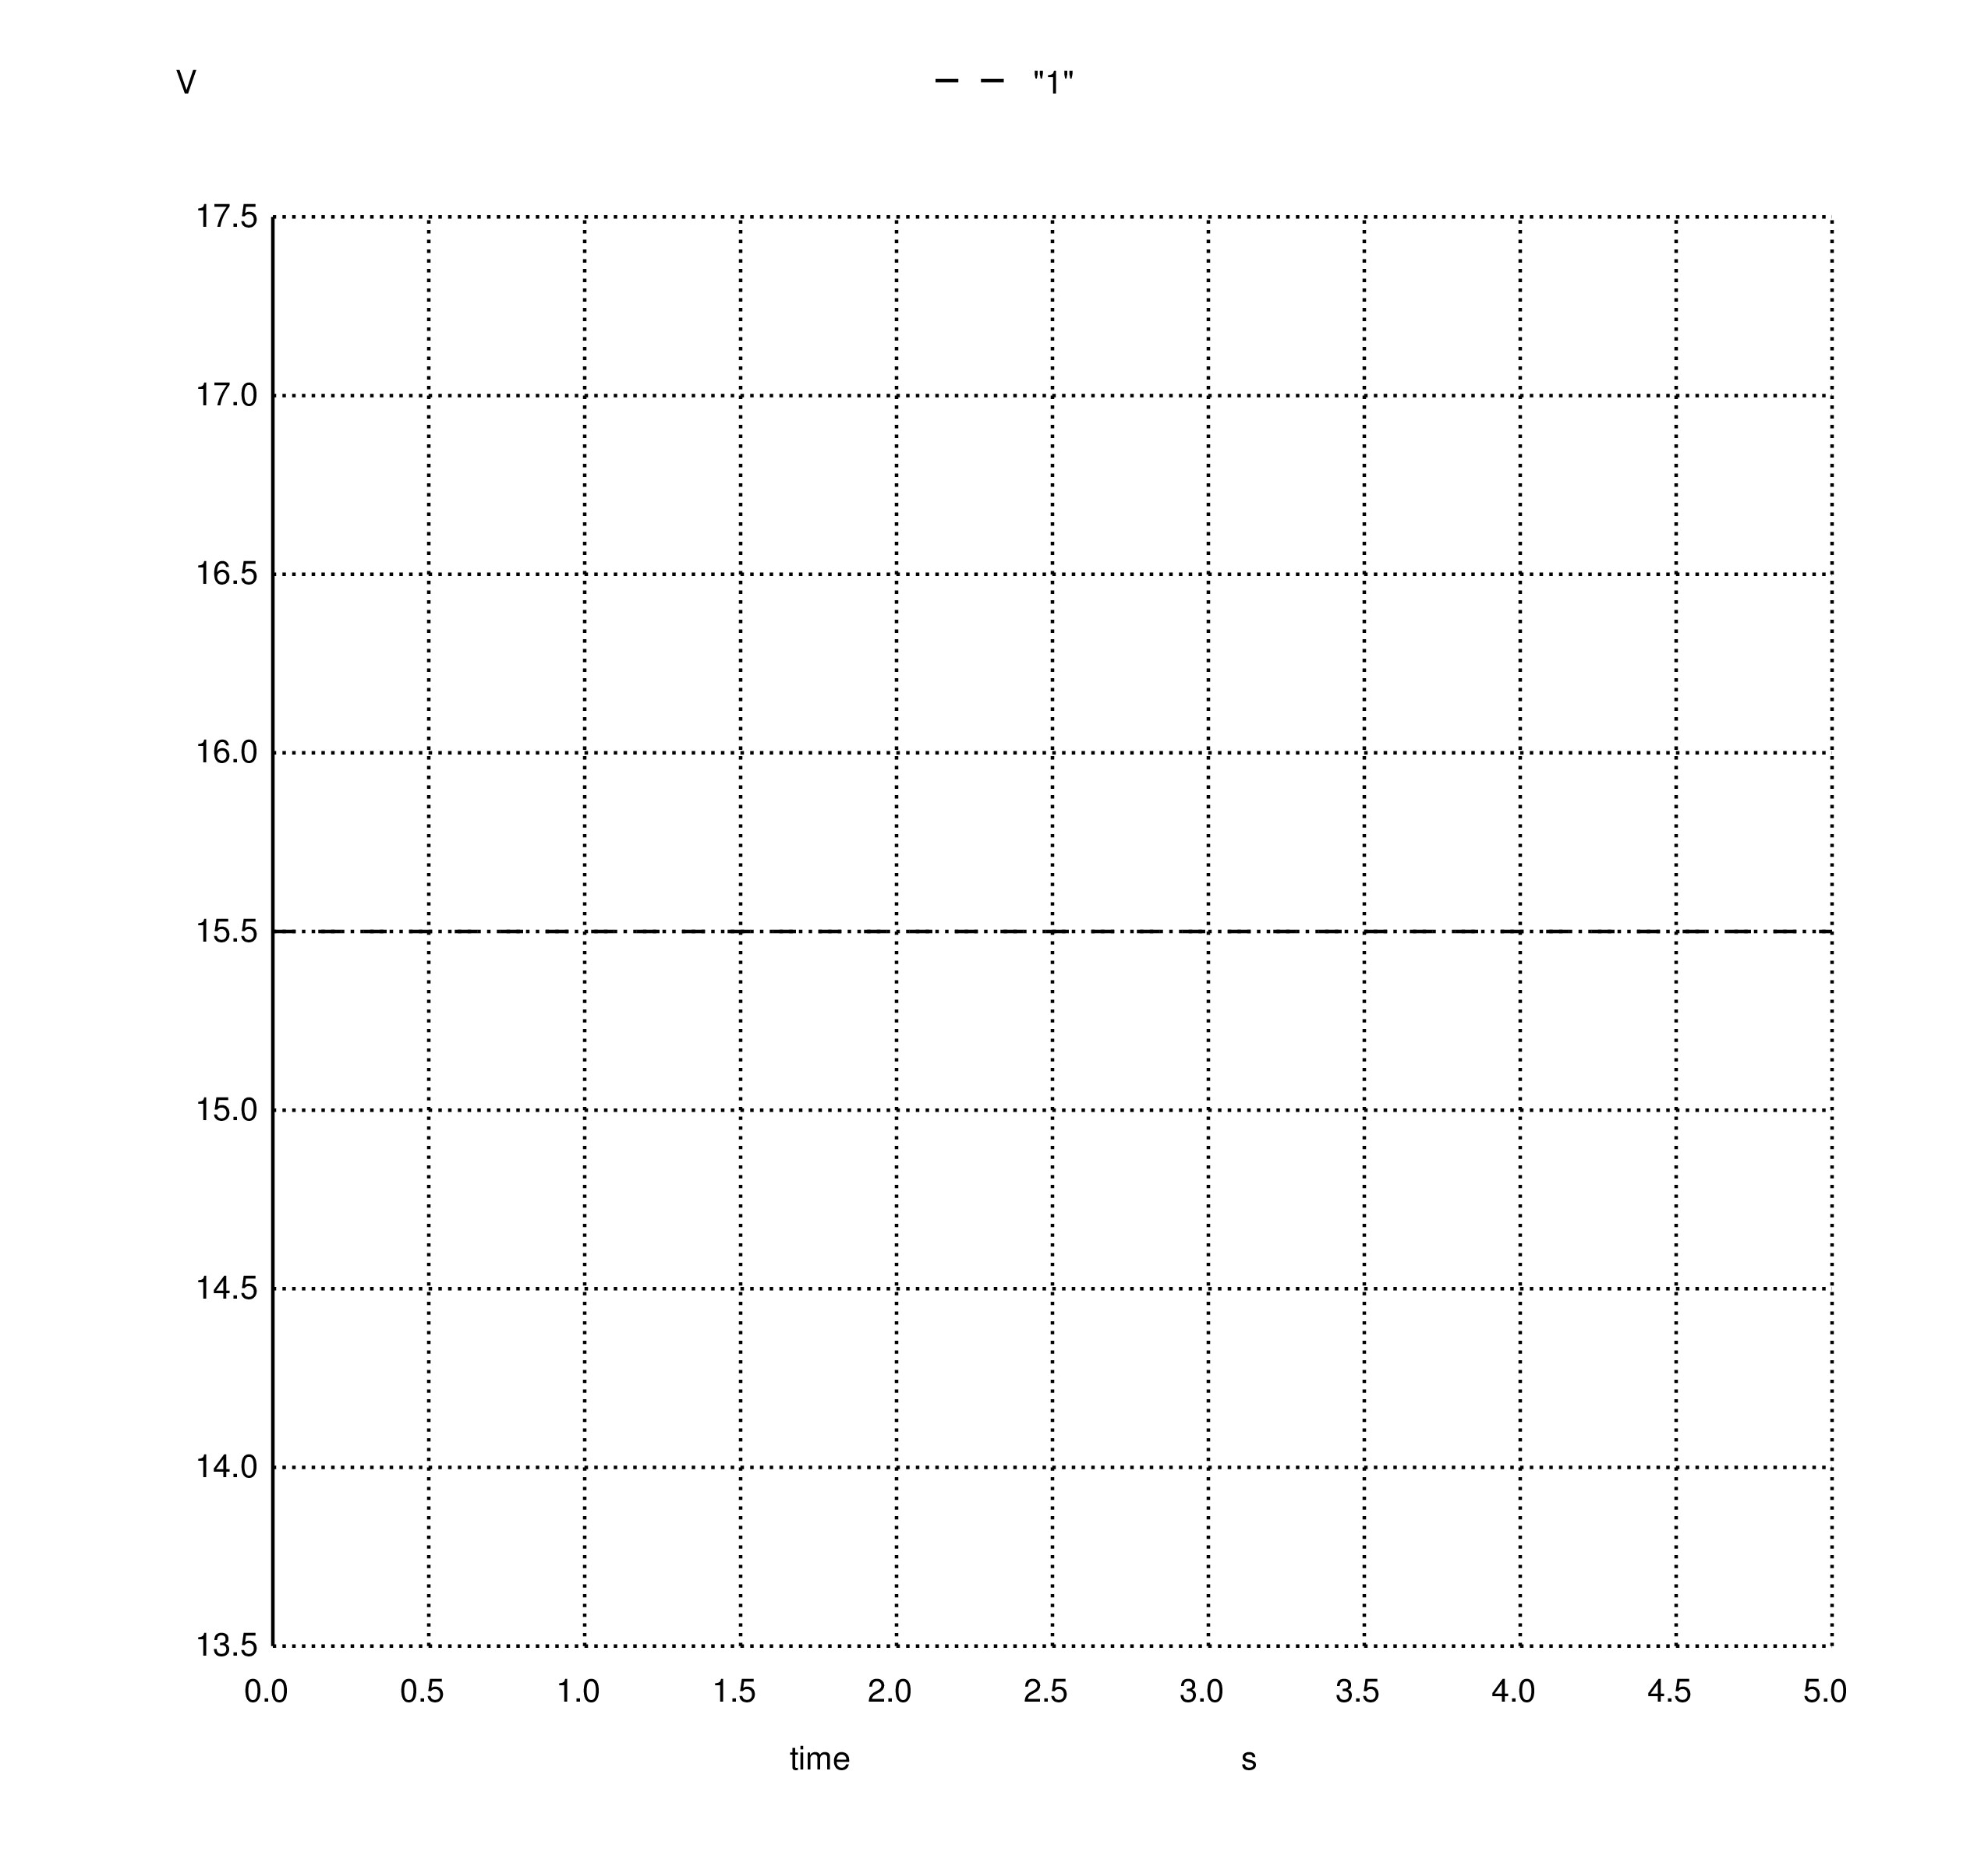
\includegraphics[width=6cm]{011.png}
\captionof{figure}{Spriegums punktā 1 uz "zemi"}
\label{att:2}
\end{minipage}%
\\
\begin{minipage}{.5\textwidth}
\centering
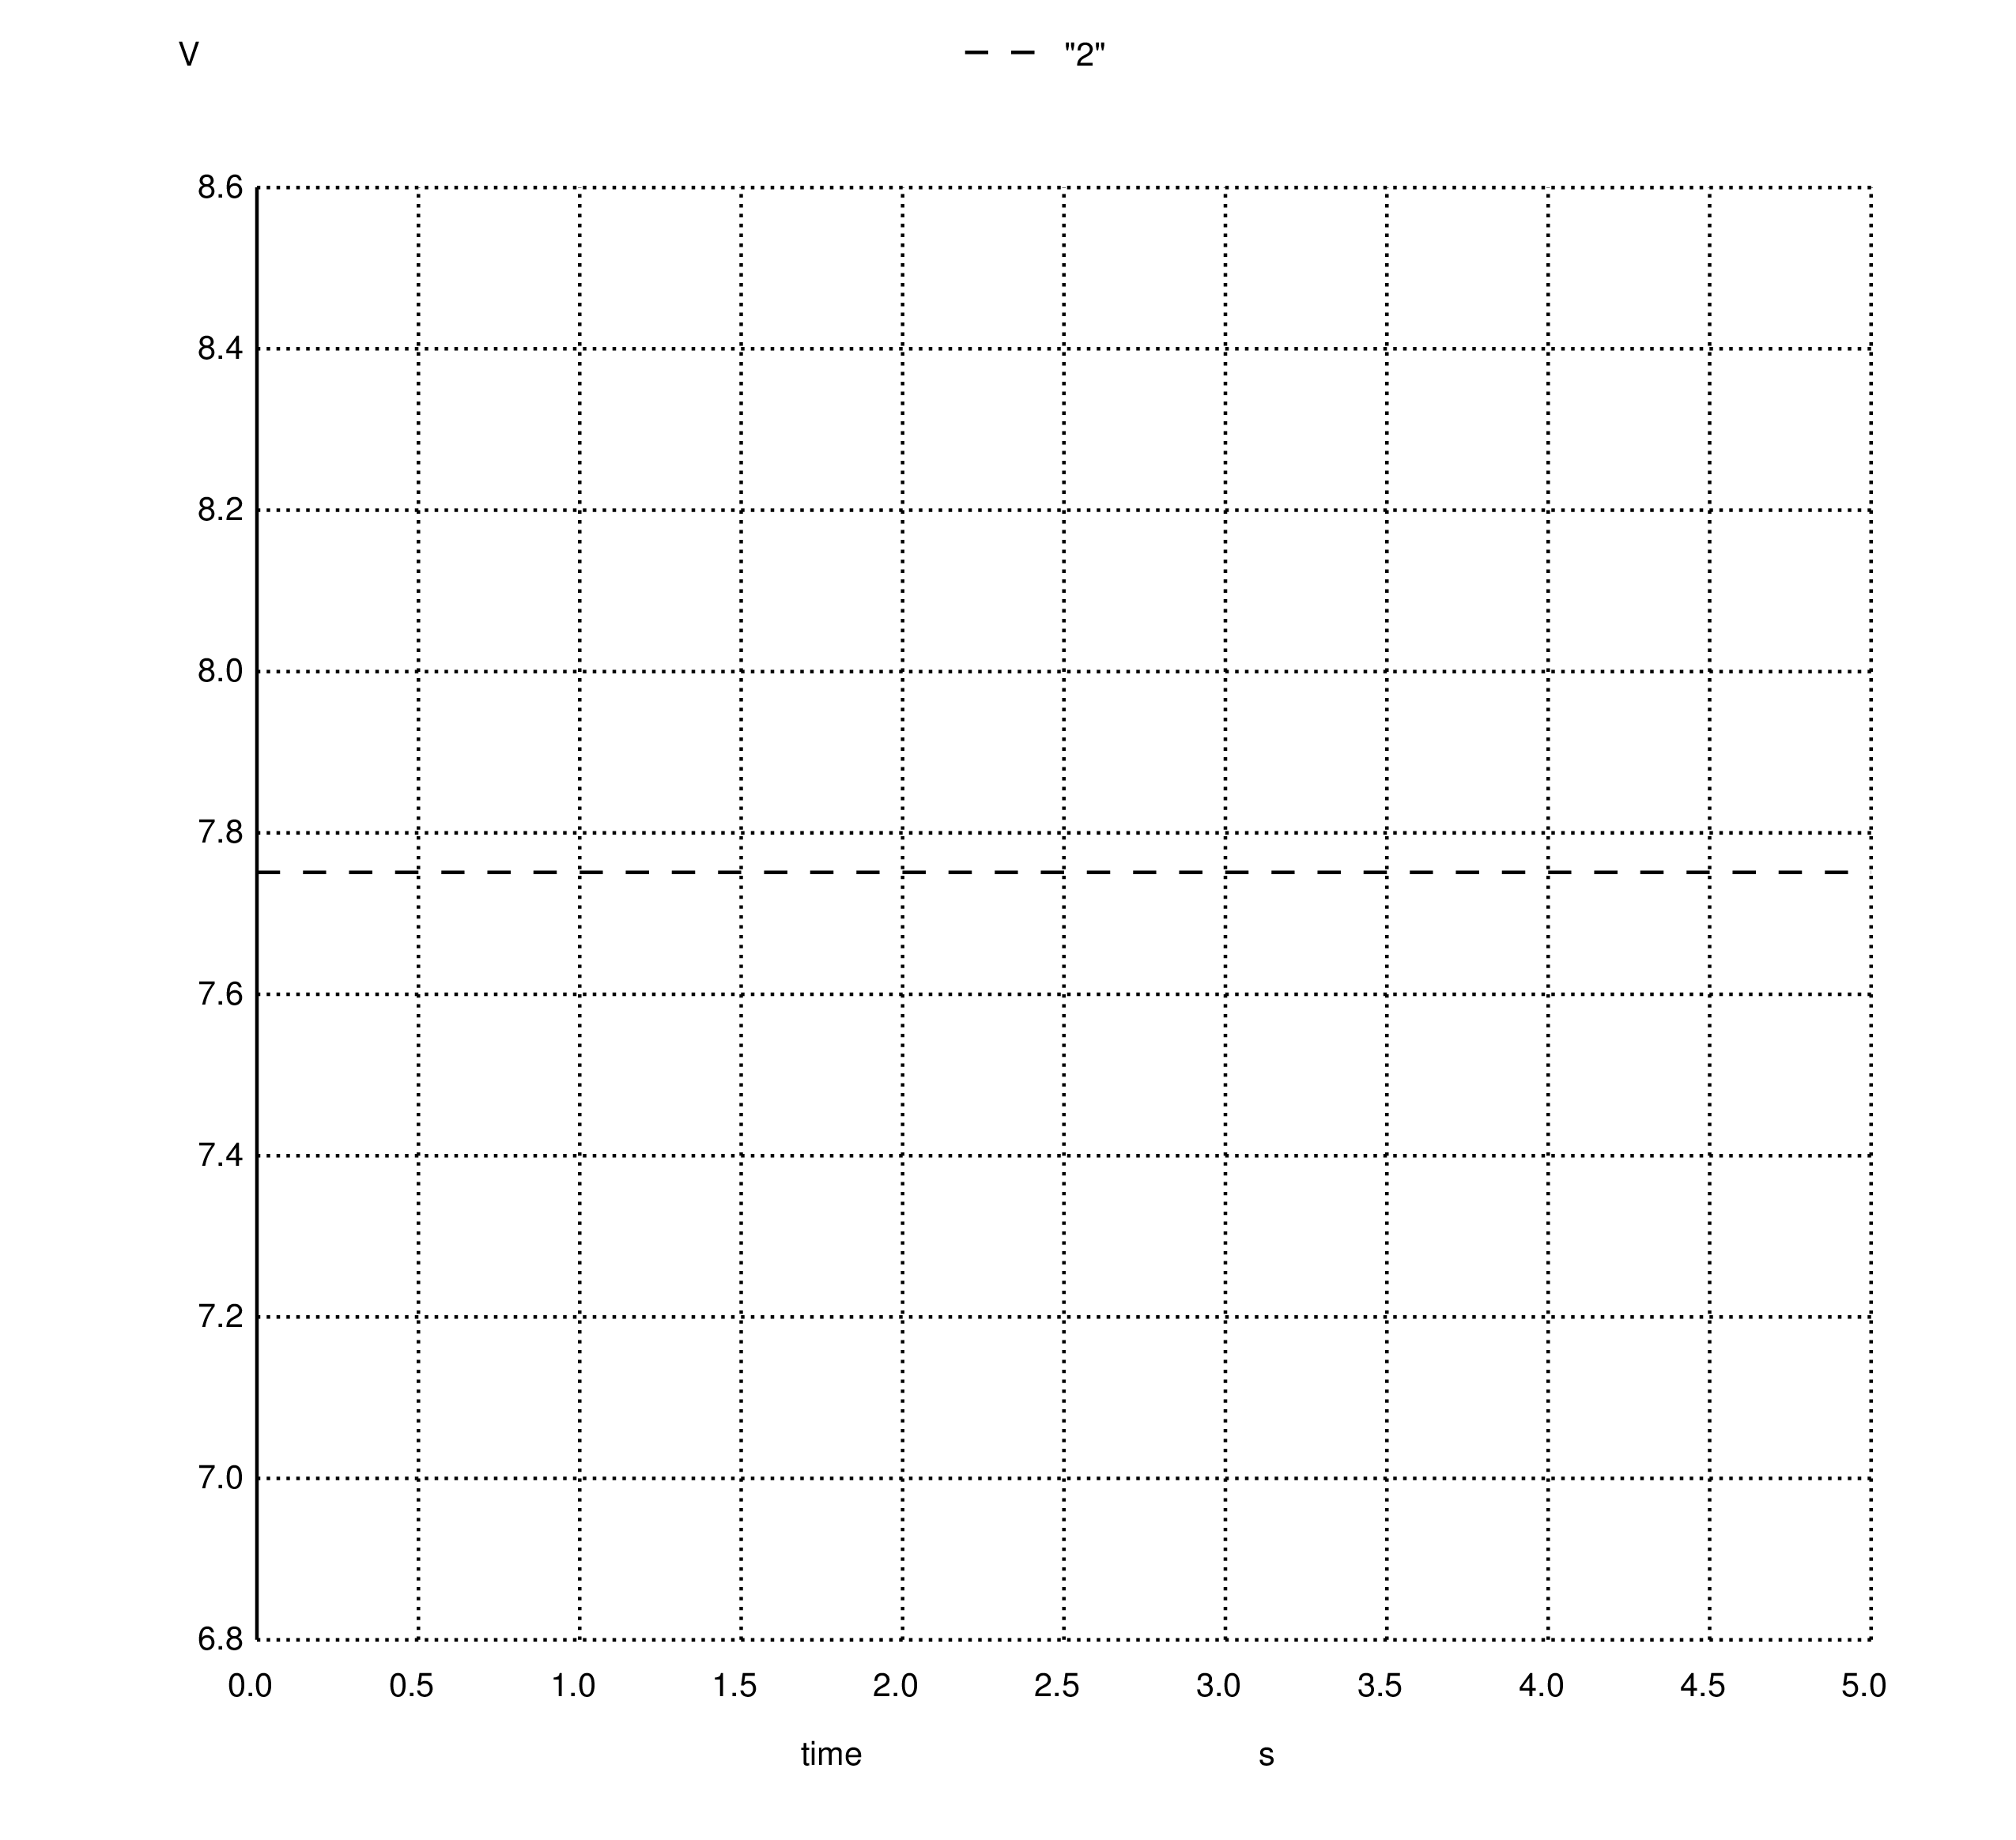
\includegraphics[width=6cm]{012.png}
\captionof{figure}{Spriegums punktā 2 uz "zemi"}
\label{att:3}
\end{minipage}
\end{figure}

\newpage
\section{Darbs ar QUCS programmām}
\subsection{Principiālā shēma}
\ref{att:4} attēlā redzamā shēma izveidota pēc dotās ķēdes,  sprieguma avota(V1) vērtība ir 15.5V, rezistoru(R1 un R2) vērtības ir 6$\Omega$.

\begin{figure}[b!]
\centering
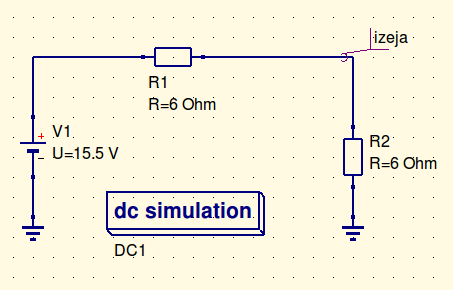
\includegraphics[scale=0.79]{prshema.png}
\captionof{figure}{}
\label{att:4}
\end{figure}

\subsection{DC simulācijas rezultāti}
Kā redzams \ref{att:5} attēlā, pēc simulācijas, eksperimentālie rezultāti sakrīt ar teorētiski izrēķinātajiem, jeb spriegumi uz abiem rezistoriem ir 7.75V.

\begin{figure}[b!]
\centering
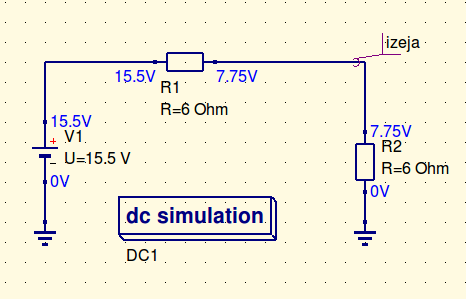
\includegraphics[scale=0.65]{dcsim.png}
\captionof{figure}{}
\label{att:5}
\end{figure}

\subsection{Sweep simulāciju rezultāti}
Sweep simulācijas shēma redzama \ref{att:6} attēlā. Pēc sweep simulācijas(\ref{att:7} att.) var redzēt, ka mainoties R2 vērtībai no 5$ \Omega$ līdz 50$ \Omega$ spriegums izejas punktā palielinās atkarībā no R2 vērtības. Jo lielāka R2 vērtība, jo lielāks izejas spriegums. 
\begin{figure}[b!]
\centering
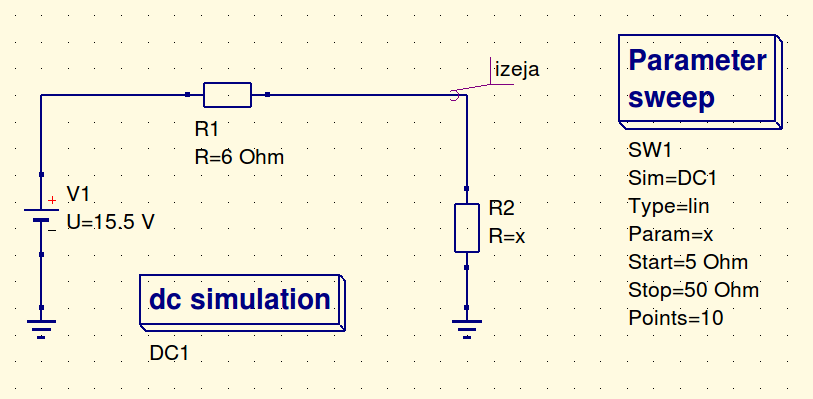
\includegraphics[scale=0.5]{swesh.png}
\captionof{figure}{}
\label{att:6}
\end{figure}

\begin{figure}[b!]
\centering
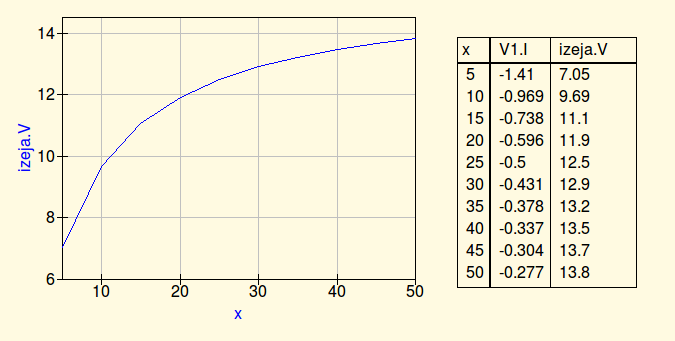
\includegraphics[scale=0.5]{swegrtb.png}
\captionof{figure}{}
\label{att:7}
\end{figure}

\chapter{Secinājumi}
\begin{itemize}
\item Šajā darbā iemācījos strādāt ar ķēžu modelēšanas programmām kā gschem, kā arī ķēžu simulācijas programmām ngspice un QUCS(kas ir arī ķēžu modelēšanas programma.).
\item Sāku mācīties un apgūt Latex\cite{latex} dokumentēšanas valodu.
\item Guvu pieredzi izmantojot online Latex valodas redaktoru "Sharelatex".
\item Veicu pirmā laboratorijas darba atskaiti.
\end {itemize}
\begin{thebibliography}{1}
\bibitem{Oms}
Ohm's Law, Electrical Math and Voltage Drop Calculations (Revised Edition) by Tom Henry (December 1, 1992)
\bibitem{latex}
LaTeX Beginner's Guide by Stefan Kottwitz (March 21, 2011)

\end{thebibliography}
\end{document}
